\section{Network formation}
\label{network_formation}

When running both the simulations the ideal result should be a Minimum Spanning Tree (MST), where there are no cycles and each vertex is connected by the shortest possible path, optimizing all the paths that start from SP considered as root of the MST.
While it's very straightfoward to use a global algorithm to calculate and draw the MST, both the simulations run using only local rules (respecting the definition of CA) and the cells' individual behaviour creates paths that are not always the best. The result for both the CAs is always a spanning tree nonetheless, although never a minimum one.

\par
The results of the two simulations are compared with one of the correct MST for two different network maps in figure~\ref{fig:mst_20_40}.

\begin{figure}[H]
    \centering
    \subfigure[MST of network with 20 nodes]{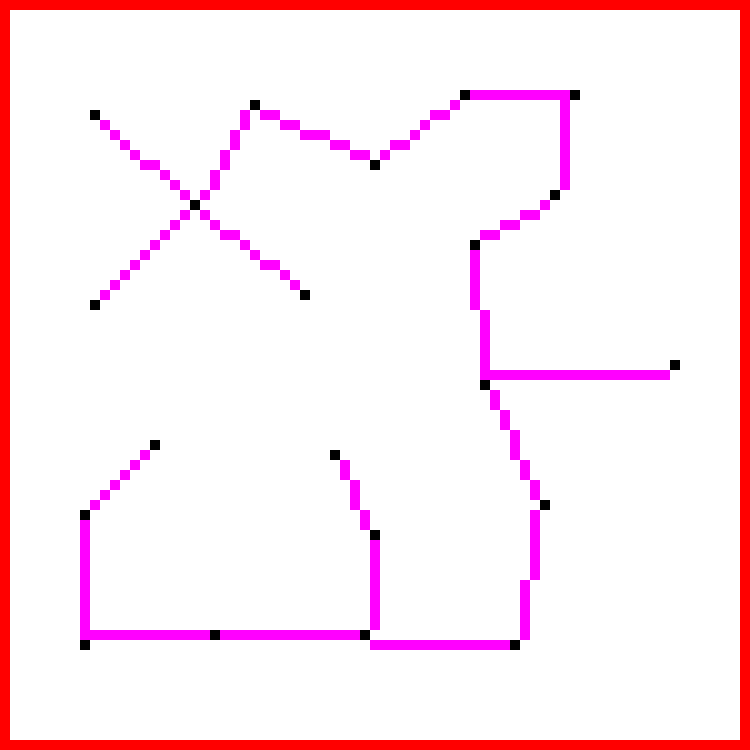
\includegraphics[width=0.32\textwidth]{mst_20}} 
    \subfigure[Paper result of simulation network with 20 nodes]{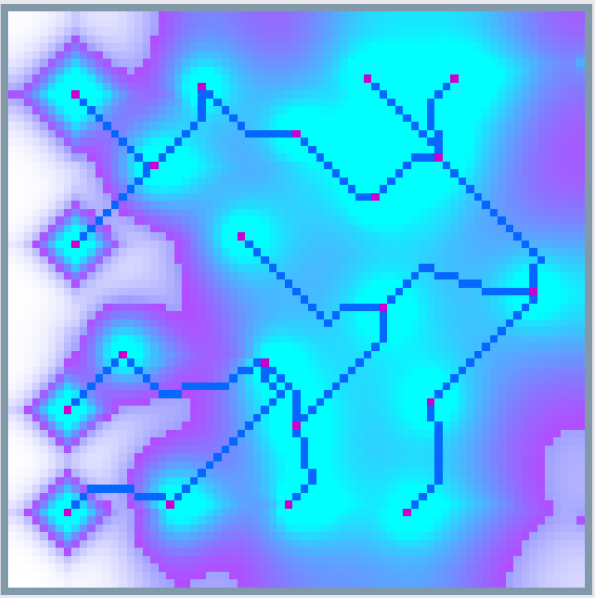
\includegraphics[width=0.32\textwidth]{wsn_20_pap/3_wsn_20}}
    \subfigure[Experimental result of simulation network with 20 nodes]{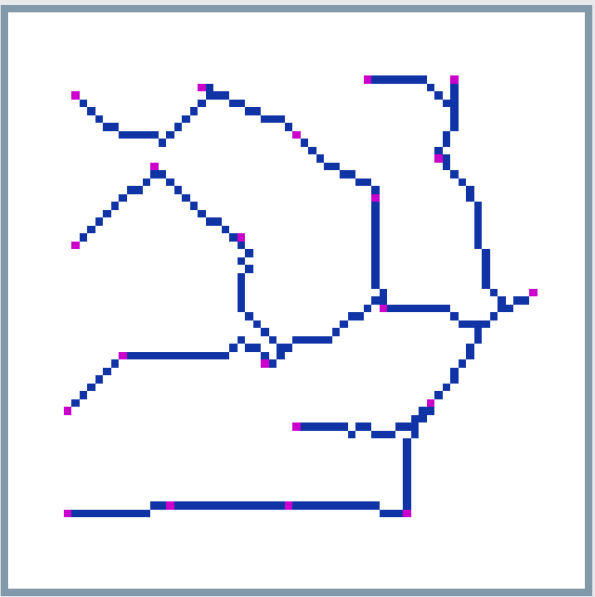
\includegraphics[width=0.32\textwidth]{wsn_20_exp/4_wsn_20}}
	
    \subfigure[MST of network with 40 nodes]{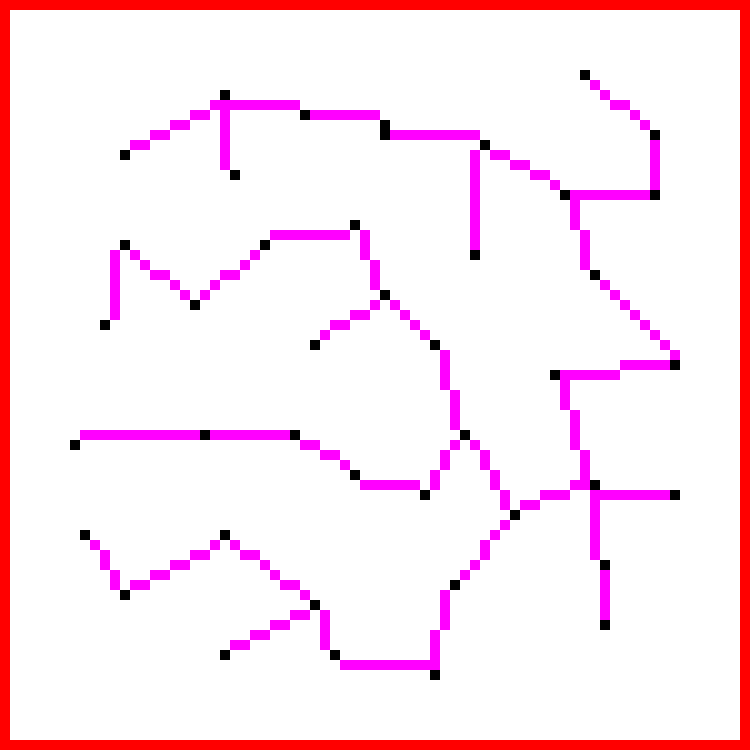
\includegraphics[width=0.32\textwidth]{mst_40}}
    \subfigure[Paper result of simulation network with 40 nodes]{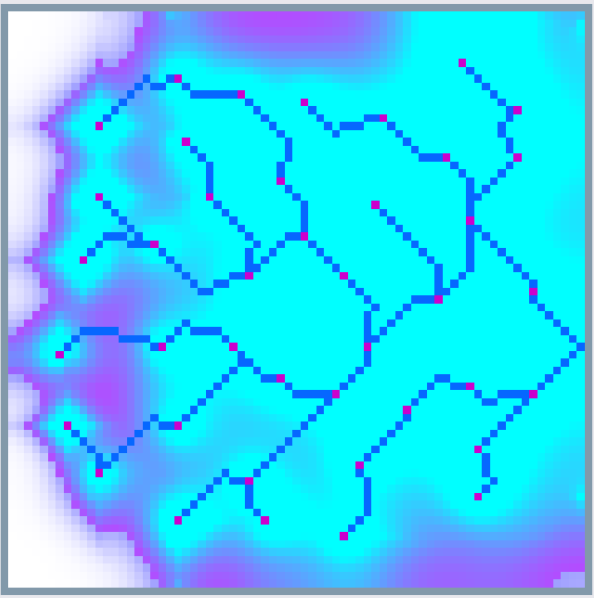
\includegraphics[width=0.32\textwidth]{wsn_40_pap/3_wsn_40}}
    \subfigure[Experimental result of simulation network with 40 nodes]{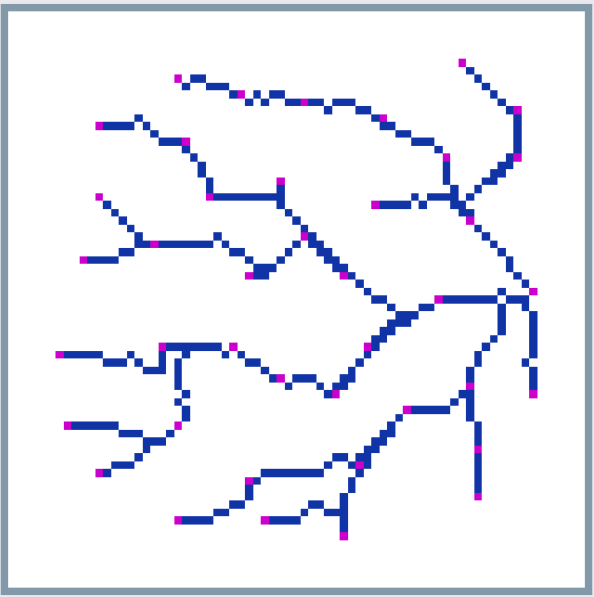
\includegraphics[width=0.32\textwidth]{wsn_40_exp/4_wsn_40}} 
    \caption{MSTs and results simulation comparison for network formation}
    \label{fig:mst_20_40}
\end{figure}

\par
First of all, we need to remember that several valid MSTs can exist for each graph depending on the order of the choices and this is one reason why some archs of the MST are different compared to the results of the simulations.

\par
The diffusion of the $PM$ to the neighbour cells following approximated rules (less accurate than the real Physarum physics) makes the gradient divert from the optimal shortest paths.
Finally another reason why the results differ from the MST is parallelism: any standard MST algorithm searches sequentially the nearest node to add it to the tree, while CAs expand in different locations at the same time because every cell is indipendent from the others. This difference makes some nodes easier to reach even if they are not the nearest from a MST point of view.

\par
For most of the time, the experimental simulation produces archs that are more similar to the MST respect to the paper simulation. For each map a better tuning of the parameters could be made to minimize this error but in all our tests our simulation outperforms the other one.

\par
From laboratory observations, when the Physarum produces his network tubes it's pretty common that two or more tubes share a part to minimize the needed mass, as can be seen in figure~\ref{fig:tube_intersection_red}.

\begin{figure}[H]
  \centering
    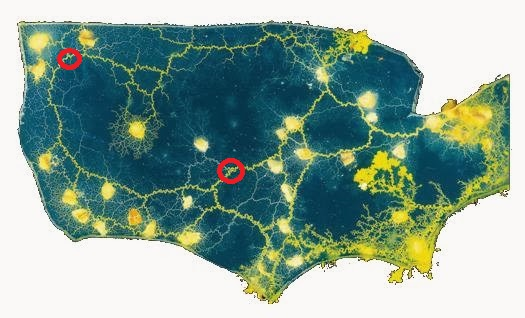
\includegraphics[width=0.48\textwidth]{tube_intersection_red}%
    
  \caption{Tubes intersection in real Physarum}
  \label{fig:tube_intersection_red}
\end{figure}

\par
The paper simulation has never showed this behaviour, creating always clean and completely separated tubes for each different couple of nodes. On the other side, the experimental simulation often produces this kind of interconnected tubes as showed in figure~\ref{fig:wsn_40_red_intersection}.

\begin{figure}[H]
  \centering
    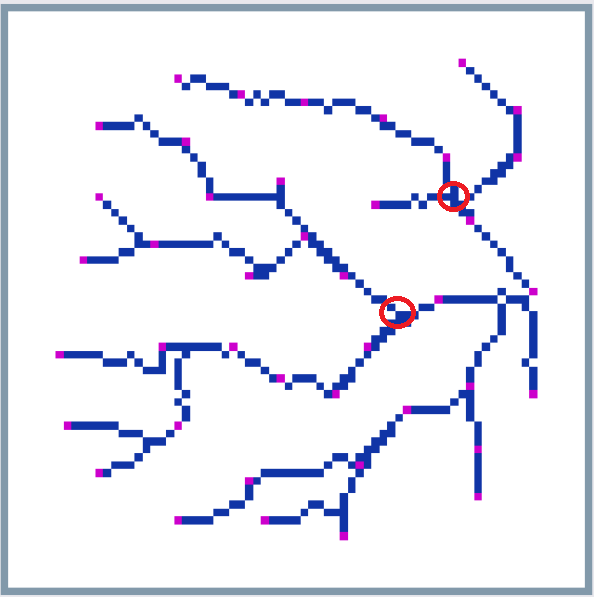
\includegraphics[width=0.48\textwidth]{wsn_40_red_intersection}%
    
  \caption{Tubes intersection in simulated Physarum}
  \label{fig:wsn_40_red_intersection}
\end{figure}

\par
The paper simulation creates his network leaving the map flooded with mould mass everywhere (as seen in figures of section \nameref{network_formation_5}), while our algorithm pushes the dispersed mass towards the tubes, leaving only the network visible as the real Physarum does. For enough large maps with NSs too far from SP, the paper algorithm crashes: as it doesn't respect the mass conservation, some cells reach a mass value so high that it overflows. A solution could be creating a limit value for the mass but in this case a lot of cells (firstly the ones near the margins of the map) would all reach the same limit value, destroying the gradient needed for connecting the NSs with SP.
If our experimental algorithm cannot reach too far NSs, the solution is to simply increase the inizial mould mass so it will be able to expand further. This makes the algorithm very robust and has never crashed during the simulations.

\par
For all these reasons, our experimental model can be considered much more solid and more similar to Physarum's real dynamics, even if we would need more laboratory pictures of all the topologies that the mould can create for a better validation process.

\section{Maze solving}

Maze solving finding the shortest path among all the possibilities is another task in which Physarum always successes. The computer simulations should also be able to solve this task in a very similar manner.

\par
In \cite{Tsompanas2016} the authors explicity say that their updated version of the algorithm is also able to solve mazes without showing any proof of that. Implementing their mathematical equations and the mould behaviour didn't get the results we were looking for: their model cannot solve mazes, even with very high PM value because of similar problems described in \nameref{network_formation}, like loosing the mass gradient when reaching the objective.

\par
We implemented two standard and famous mazes used as examples in Physarum scientific documentation and only the experimental model was able to solve them. The failed attempts of the paper simulation are shown in figures of section \nameref{maze_solving} (subsection \nameref{paper_model}).
Giving enough mass to the mould, the experimental model was able to find the shortest path in every maze as shown in \nameref{maze_solving} (subsection \nameref{experimental_model}), reaching the optimal solution every single time.

\par
If we don't strictly consider the possible routes inside the maze but instead the single cells of the map then the simulation often returns a suboptimal solution with an epsilon error respect to the absolute shortest path as can be seen in figure~\ref{fig:mst_tube}.

\begin{figure}[H]
    \centering
    \subfigure[MST of second maze]{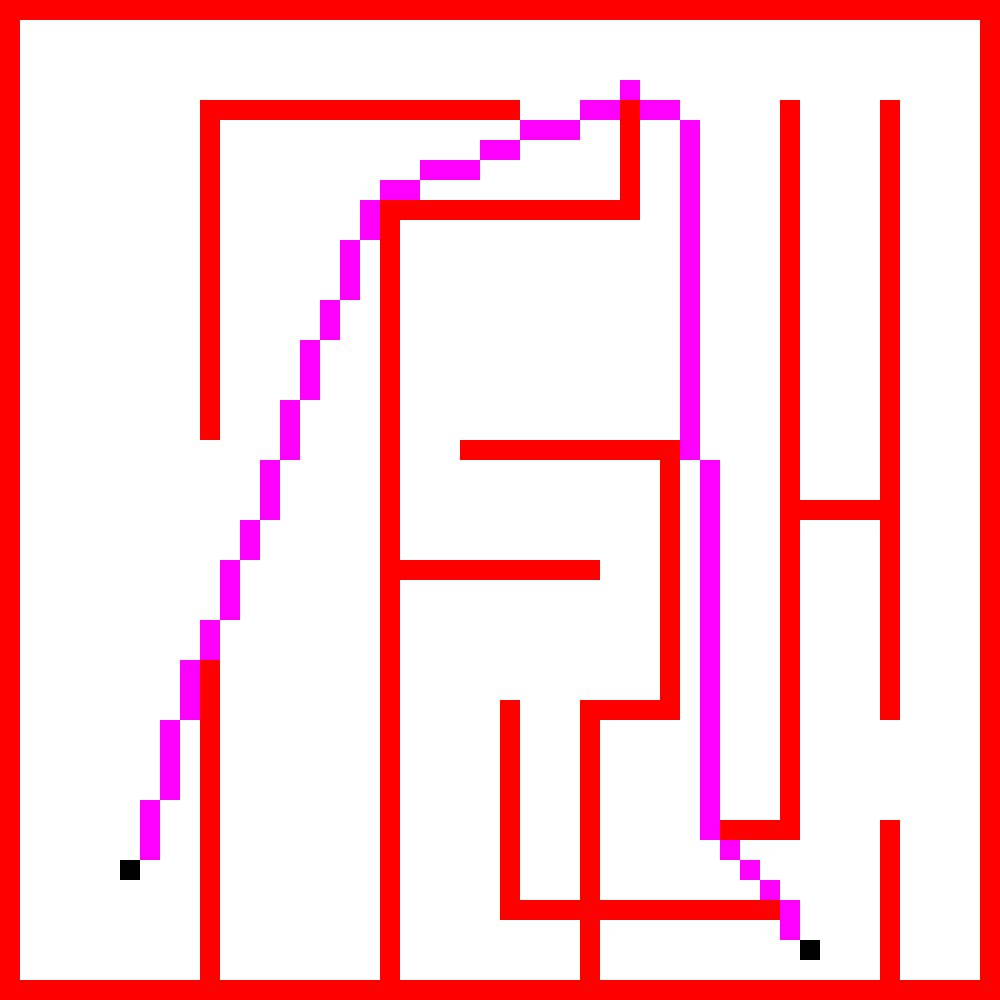
\includegraphics[width=0.32\textwidth]{mst_tube}}
    \subfigure[Paper result of second maze]{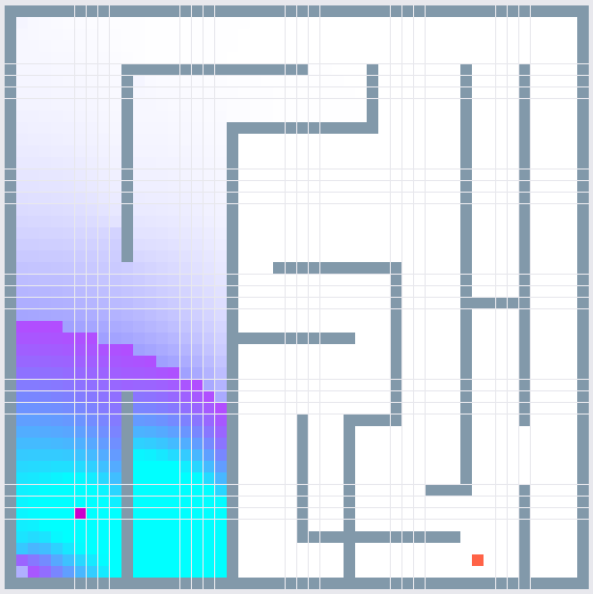
\includegraphics[width=0.32\textwidth]{generic_maze_pap/3_generic_maze}} 
    \subfigure[Experimental result of second maze]{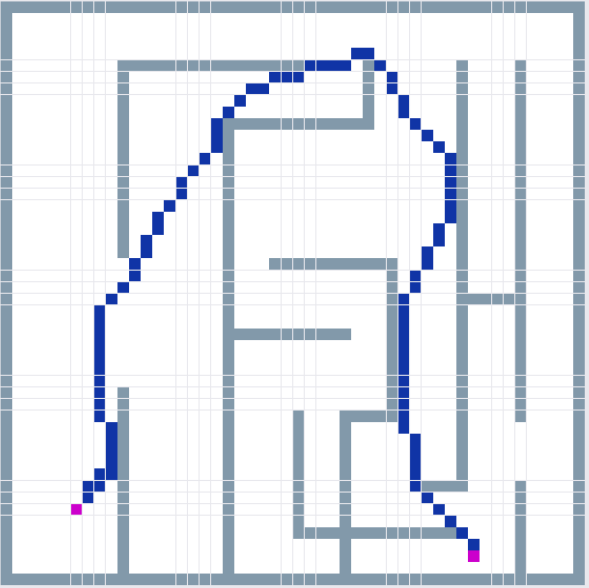
\includegraphics[width=0.32\textwidth]{generic_maze_exp/4_generic_maze}} 
    \caption{MST and results simulation comparison for maze solving}
    \label{fig:mst_tube}
\end{figure}

\par
The cause is the distribution of mass in cells instead of a continuos space: the gradient used to draw the tube is pseudorandomly moved to the pixels near the optimal solution, in a similar fashion to the network archs in section \nameref{network_formation}.

\par
Both the real mould and our experimental model reach the target in the maze with the best possible path, leaving no other useless mass around the map, therefore our CA is validated also for this task.
